\subsection{Network Devices}

\begin{frame}{Network devices in Linux}
	\begin{itemize}
		\item In UNIX systems, the common saying is that "\textit{everything is a file}"
		\item Most classes of devices follow that rule, and expose \textbf{block} and \textbf{char} devices in \code{/dev}
			\begin{itemize}
				\item \code{/dev/mmcblk0} : eMMC device 0
				\item \code{/dev/i2c-3} : I2C bus number 3
				\item \code{/dev/input/*} : HID devices
			\end{itemize}
		\item Network devices don't follow that rule, as they are rarely directly accessed
		\item The Linux Kernel provides access to Layers 2, 3 and 4 through the \textbf{socket} API
		\item Network devices appear as \textbf{interfaces} under \code{/sys/class/net}
		\item The \code{sysfs} API is only for limited control and device information
	\end{itemize}
\end{frame}

\begin{frame}{\code{struct net_device}}
	\begin{itemize}
		\item The \kstruct{net_device} structure represents a conduit
		\item Used for \textbf{physical} interfaces and \textbf{virtual} interfaces
		\item Abstract interfaces can be used for \textbf{vlan}, \textbf{bridging}, \textbf{tap}, \textbf{veth}, etc.
		\item Every \kstruct{net_device} object can transmit and receive packets :
			\begin{itemize}
				\item Physically, in which case it is managed by a device driver
				\item or Logically, by passing them to another component in the stack after potentially altering them
			\end{itemize}
		\item Instances of \kstruct{net_device} are often called \code{netdev} in the Documentation
		\item Variables of that type are usually named \code{dev}
			\begin{itemize}
				\item Unfortunately, this is als the usual name of \kstruct{device} objects
			\end{itemize}
	\end{itemize}
\end{frame}

\begin{frame}{\code{struct net_device} (2)}
	\begin{itemize}
		\item Userspace sees a \code{netdev} as an \textbf{interface}
			\begin{itemize}
				\item Listed with \code{ip link show} or \code{ifconfig}
				\item Also appearing under \code{/sys/class/net/}
			\end{itemize}
		\item Interfaces have a \textbf{name}, which may change
		\item Interfaces also have an index (\textbf{ifindex}) that uniquely identifies them
		\item They have attributes, changeable or not, depending on their type :
			\begin{itemize}
				\item Addresses : IPv4, IPv6, MAC, etc.
				\item Properties : MTU, Queue length, etc.
				\item Statistics : RX/TX packets, link events, etc.
				\item State : Link up or down, admin state, Promiscuous, etc.
			\end{itemize}
	\end{itemize}
\end{frame}

\begin{frame}[fragile]{Network driver}
	\begin{itemize}
		\item Creating a new Network Interface driver is similar to any other driver :
			\item The driver registers a \textbf{device driver} on its underlying bus :
				{\fontsize{6}{7}\selectfont
				\begin{minted}[bgcolor=lightgray!40]{c}
static const struct of_device_id mvneta_match[] = {
        { .compatible = "marvell,armada-3700-neta" },
        { }
};

static struct platform_driver mvneta_driver = {
        .probe = mvneta_probe,
        .remove = mvneta_remove,
        .driver = {
                .name = MVNETA_DRIVER_NAME,
                .of_match_table = mvneta_match,
        },
};
module_platform_driver(mvneta_driver);
				\end{minted}
				}
			\item In the \code{.probe()} function, allocate a \kstruct{net_device} :
				{\fontsize{6}{7}\selectfont
				\begin{minted}[bgcolor=lightgray!40]{c}
dev = devm_alloc_etherdev_mqs(&pdev->dev, sizeof(struct mvneta_port),
                              txq_number, rxq_number);
				\end{minted}
					}
			\item The \code{netdev} is \textbf{registered} to the networking subsystem :
				{\fontsize{6}{7}\selectfont
				\begin{minted}[bgcolor=lightgray!40]{c}
register_netdev(dev);
				\end{minted}
				}
	\end{itemize}
\end{frame}

\begin{frame}{Reminder - Device Model and Device Drivers}
  \begin{columns}
    \column{0.7\textwidth} In Linux, a driver is always interfacing
    with:
    \begin{itemize}
    \item a {\bf framework} that allows the driver to expose the
      hardware features in a generic way.
    \item a {\bf bus infrastructure}, part of the device model, to
      detect/communicate with the hardware.
    \end{itemize}
    \column{0.3\textwidth}
    \includegraphics[height=0.8\textheight]{slides/networking-stack-netdevice/driver-architecture.pdf}
  \end{columns}
\end{frame}

\begin{frame}[fragile]{Netdevice allocation}
	\begin{itemize}
		\item \kfunc{alloc_netdev_mqs} : Main allocation function :
			{\fontsize{8}{7}\selectfont
			\begin{minted}{c}

struct net_device *
alloc_netdev_mqs(int sizeof_priv,                /* Size of driver-dedicated private data area */
                 const char *name,               /* Default name of the device */
                 unsigned char name_assign_type, /* Category of device name assignment */
                 void (*setup)(struct net_device *), /* Setup callback function */
                 unsigned int txqs,              /* Number of TX queues */
                 unsigned int rxqs);             /* Number of RX queues */
			\end{minted}
			}
		\item The \code{setup} callback is called directly by \kfunc{alloc_netdev_mqs}
		\item \kfunc{free_netdev} is used to destroy the netdevice
		\item \textbf{device-managed} variants exist : \kfunc{devm_alloc_etherdev_mqs}
	\end{itemize}
\end{frame}

\begin{frame}{Netdevice naming}
	\begin{itemize}
		\item Netdevice names can be changed dynamically, and the name source is tracked
		\item \code{dev->name_assign_type}, exposed in \code{/sys/class/net/xxx/name_assign_type}
		\item \code{NET_NAME_ENUM} : Name built sequentially by the kernel 
			\begin{itemize}
				\item e.g. \code{eth0, eth1}, etc.
			\end{itemize}
		\item \code{NET_NAME_PREDICTABLE} : Name predictably assigned by the kernel
			\begin{itemize}
				\item e.g. \code{label="lan1"} in devicetree for DSA switches
			\end{itemize}
		\item \code{NET_NAME_USER} : Name assigned by the user during device creation
			\begin{itemize}
				\item e.g. \code{ip link add link eth0.10 type vlan id 10}
			\end{itemize}
		\item \code{NET_NAME_RENAMED} : Device was renamed by userspace
			\begin{itemize}
				\item e.g. \code{ip link set dev eth0 name new-eth0}
				\item Used by systemd's \href{https://www.freedesktop.org/wiki/Software/systemd/PredictableNetworkInterfaceNames/}{Predictable Network Interface Names}
			\end{itemize}
	\end{itemize}
\end{frame}

\begin{frame}{Ethernet-specific device allocation}
	\begin{itemize}
		\item \kfunc{alloc_etherdev_mqs} : Allocate a new \kstruct{net_device} for Ethernet :
		\item Sets the number of queues passed as parameters
		\item Creates a default name using the \code{"eth\%d"} template
		\item Sets all the Ethernet-specific default parameters :
			\begin{itemize}
				\item MTU, Header len, Address len, etc.
			\end{itemize}
	\end{itemize}
\end{frame}

\begin{frame}[fragile]{Netdev ops}
	\begin{itemize}
		\item Before registering, the driver populates a \kstruct{net_device_ops}
	\begin{block}{mvneta.c - simplified}
		{\fontsize{8}{7}\selectfont
		\begin{minted}{c}
static const struct net_device_ops mvneta_netdev_ops = {
        .ndo_open            = mvneta_open,
        .ndo_stop            = mvneta_stop,
        .ndo_start_xmit      = mvneta_tx,
        .ndo_set_mac_address = mvneta_set_mac_addr,
        .ndo_change_mtu      = mvneta_change_mtu,
...
};

static int mvneta_probe(struct platform_device *pdev)
{
        ...
        dev->netdev_ops = &mvneta_netdev_ops;

        register_netdev(dev);
}
		\end{minted}
		}
	\end{block}
	\item These hooks are referred to as \textbf{NDO}s
	\item \code{.ndo_start_xmit} must be populated, all other are optional.
	\end{itemize}
\end{frame}

\begin{frame}{Common NDOs}
	\begin{itemize}
		\item \code{.ndo_open} and \item \code{.ndo_stop} : Bring the interface UP or DOWN
			\begin{itemize}
				\item Call when using \code{ip link set eth0 up/down}
			\end{itemize}
		\item \code{.ndo_start_xmit} : Send a packet
		\item \code{.ndo_set_rx_mode} : Configure the \textbf{rx filtering}
		\item \code{.ndo_set_mac_address} : Notify the driver that the MAC address was changed
		\item \code{.ndo_get_stats64} : Ask for hardware or driver statistics
		\item \code{.ndo_eth_ioctl} : Device-level \code{ioctl} handler, phased-out.
	\end{itemize}
\end{frame}

\begin{frame}{Netdev registration}
	\begin{itemize}
		\item \kfunc{register_netdevice} : Registers the \kstruct{net_device}, in the \code{netdev->net} namespace
			\begin{itemize}
				\item Allocates the interface index
				\item Makes the device visible from userspace
				\item From this point on, NDOs may be called
				\item Assumes \code{RTNL} is held.
				\item \code{.ndo_init} is called at that stage, if provided
			\end{itemize}
		\item \kfunc{register_netdev} : Calls \kfunc{register_netdevice} with RTNL held
			\begin{itemize}
				\item Used mostly in drivers, as the device driver's \code{.probe()} doesn't hold RTNL
			\end{itemize}
	\end{itemize}
\end{frame}

\begin{frame}{Stacking Network Devices}
	\begin{itemize}
		\item Netdevices can be independent conduits, or stacked in a hierarchy
		\item e.g. a VLAN is represented as a dedicated \code{netdev}
			\begin{itemize}
				\item A VLAN netdev's \code{lower_dev} is the physical device
				\item The physical netdev's \code{upper_dev} is the VLAN device
			\end{itemize}
		\item \kstruct{net_device} has a list of \code{lower_dev} and \code{upper_dev}
		\item Packets may be passed between netdevs, which may modify them, e.g.
			\begin{itemize}
				\item Encapsulation and Decapsulation (VLANs, tunnels)
				\item Redirection and Routing (bridges)
				\item Duplication and Redundancy (hsr, bond)
				\item Encryption (macsec, wireguard)
			\end{itemize}
		\item Can also be virtual interfaces, such as \code{veth}, \code{tun} and \code{tap}
	\end{itemize}
	\begin{center}
		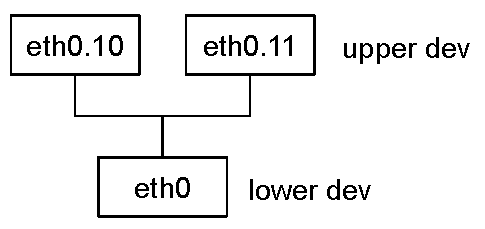
\includegraphics[width=0.3\textwidth]{slides/networking-stack-netdevice/vlan_uplow.pdf}
	\end{center}
\end{frame}

\begin{frame}[fragile]{Stacking Network Devices - 2}
	\begin{itemize}
		\item Stacked devices show in userspace as \code{dev@lower}
			\begin{itemize}
				\item \textit{e.g.} DSA ports show as \code{lan1@eth0}
				\item DSA uses stacking for the \textbf{conduit} interface
			\end{itemize}
		\item The relationship is declared by calling :
			\begin{minted}{c}
int netdev_upper_dev_link(struct net_device *dev,
                          struct net_device *upper_dev,
                          struct netlink_ext_ack *extack)
			\end{minted}
		\item A \code{netdev} can also have a \code{master} device
			\begin{itemize}
				\item Similar to \textbf{upper}, except a \code{netdev} can only have one master
				\item Used for \textbf{bridges}
				\item \code{ip link set dev eth0 master br0}
			\end{itemize}
	\end{itemize}
\end{frame}

\begin{frame}{Network Namespaces}
	\begin{itemize}
		\item Netdevs can only view and pass traffic to other netdevs in the same \textbf{namespace}
		\item Net Namespaces, or \textbf{netns}, are represented internally by \kstruct{net}
		\item A \code{netns} is created using \code{netlink}, e.g. through \code{iproute2} :
			\begin{itemize}
				\item \code{ip netns add new_netns}
			\end{itemize}
		\item Network namespace have their own set of resources :
			\begin{itemize}
				\item Routing tables, ARP tables, caches, pools of memory, identifier pools...
			\end{itemize}
		\item Netdevs are \textbf{moved} to a \code{netns} with \code{ip link set dev eth0 netns new_netns}
		\item All \code{netns} contain a \textbf{loopback} interface named \code{lo}, created when netdev is added to the netns
		\item Dedicated mechanisms such as \textbf{veth pairs} must be used for inter-netns communication
		\item Used by Containers for isolation
	\end{itemize}
\end{frame}

\begin{frame}{Network Namespaces - 2}
	\begin{itemize}
		\item User processes run within a given \textbf{netns} and cannot see other interfaces
			\begin{itemize}
				\item \code{ip netns <ns> exec <cmd>} : Run \code{cmd} in the \code{ns} namespace
			\end{itemize}

		\item By default, netdevs are created in the \textbf{init\_ns}
	\end{itemize}
	\begin{center}
	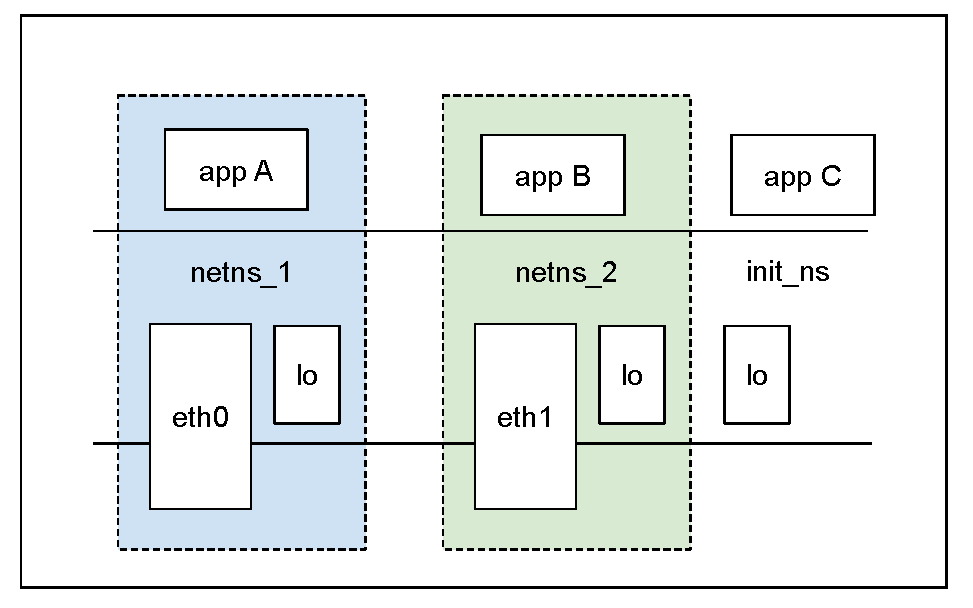
\includegraphics[width=0.7\textwidth]{slides/networking-stack-netdevice/netns.pdf}
	\end{center}
\end{frame}

\begin{frame}{\code{veth} : Virtual Ethernet Pairs}
	\begin{itemize}
		\item \code{ip link add type veth} : creates \code{veth0@veth1} and \code{veth1@veth0}
		\item Both \code{veth0} and \code{veth1} are linked together, traffic flows between the 2
		\item Main way to traverse namespaces, heavily used by containers
	\end{itemize}
	\begin{center}
	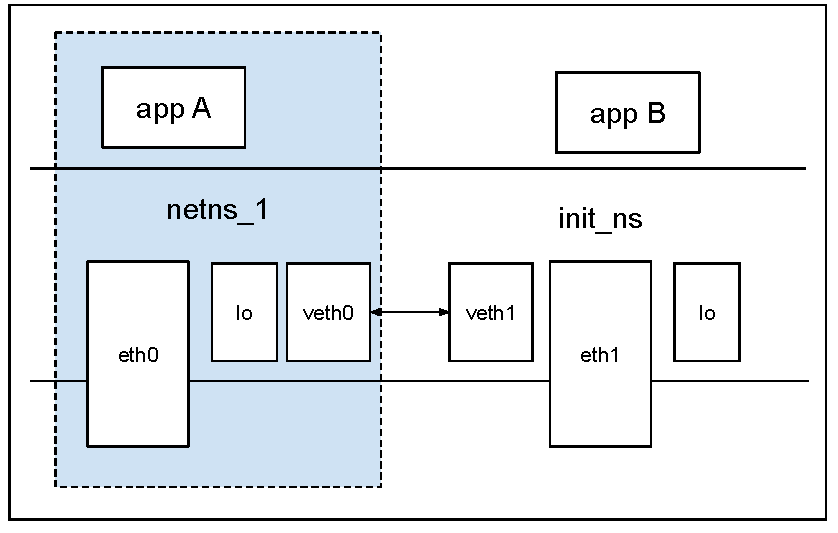
\includegraphics[width=0.6\textwidth]{slides/networking-stack-netdevice/veth.pdf}
	\end{center}
\end{frame}

\begin{frame}{Bridges}
	\begin{center}
	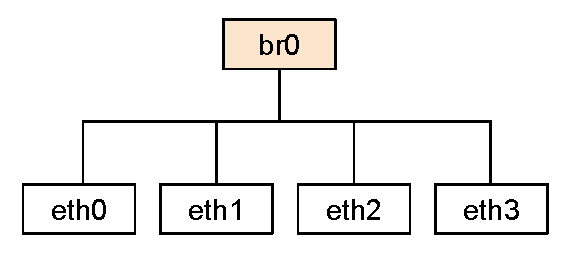
\includegraphics[width=0.4\textwidth]{slides/networking-stack-netdevice/bridge.pdf}
	\end{center}
	\begin{itemize}
		\item A \textbf{bridge} represents a logical switch.
		\item If there is a hardware switch, its ports should act as \textbf{standalone} interfaces
			\begin{itemize}
				\item A logical switch corresponding to the hardware can be re-created
				\item switching operations can be \textbf{offloaded} in hardware with \textbf{switchdev}
			\end{itemize}
		\item Bridges are represented with their own \kstruct{net_device}
			\begin{itemize}
				\item Created with \code{ip link add name br0 type bridge}
				\item It acts as the \textbf{master} of all the switch ports
				\item Ports are added with {ip link set dev lan0 master br0}
			\end{itemize}
		\item The bridge interface maintains the \code{fdb} and handles forwarding
	\end{itemize}
\end{frame}

\begin{frame}{Vlan}
	\begin{itemize}
		\item Multiple types of Vlans are supported in Linux through dedicated drivers
		\item 802.1Q : Layer 2 tag-based VLANs
			\begin{itemize}
				\item \code{ip link add link eth0 name eth0-100 type vlan id 100}
			\end{itemize}
		\item 802.1AD (Q in Q) : Allows using Vlans within Vlans, with multiple tags
			\begin{itemize}
				\item \code{ip link add link eth0 name eth0-100 type vlan id 100 protocol 802.1ad}
			\end{itemize}
		\item VxLAN : VLAN using UDP encapsulation
			\begin{itemize}
				\item \code{sudo ip link add link eth0 name vxlan100 type vxlan id 100 \ }
					\code{local 192.168.42.1 remote 192.168.42.2}
			\end{itemize}
		\item MACVlan : Virtual interface with a different MAC address than the physical one
			\begin{itemize}
				\item \code{ip link add macvlan1 link eth0 type macvlan mode bridge}
				\item Used a lot by containers
			\end{itemize}
	\end{itemize}
\end{frame}

\begin{frame}{tun and tap interfaces}
	\begin{columns}
	\column{0.4\textwidth}
	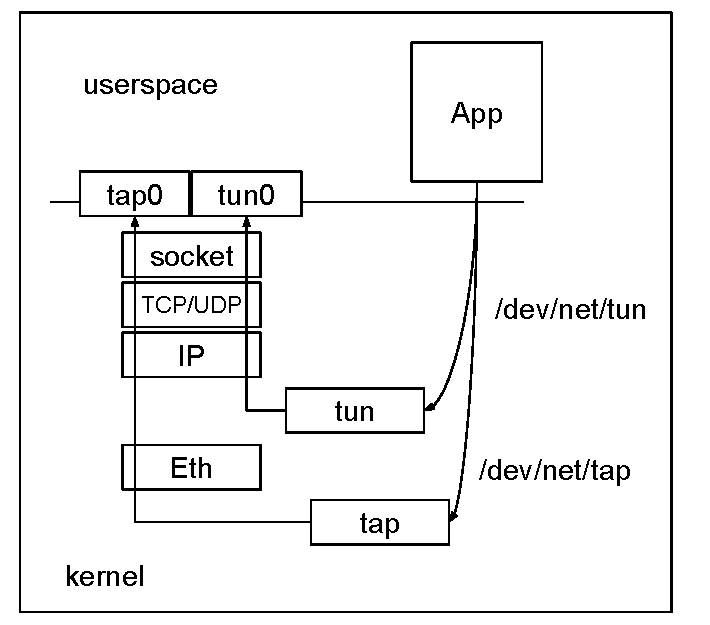
\includegraphics[width=\textwidth]{slides/networking-stack-netdevice/tuntap.pdf}
	\column{0.6\textwidth}
	\begin{itemize}
		\item Create virtual interfaces where a userspace program feeds and receives data from the \code{netdev}
			\begin{itemize}
				\item Data is sent and received by accessing \code{/dev/net/tun}
			\end{itemize}
		\item Used for userspace tunnel implementations, such as VPNs
		\item \code{ip tuntap add dev tun0 mode tun}
		\item \code{ip tuntap add dev tap0 mode tap}

	\end{itemize}
	\end{columns}
\end{frame}

